\documentclass[1p]{elsarticle_modified}
%\bibliographystyle{elsarticle-num}

%\usepackage[colorlinks]{hyperref}
%\usepackage{abbrmath_seonhwa} %\Abb, \Ascr, \Acal ,\Abf, \Afrak
\usepackage{amsfonts}
\usepackage{amssymb}
\usepackage{amsmath}
\usepackage{amsthm}
\usepackage{scalefnt}
\usepackage{amsbsy}
\usepackage{kotex}
\usepackage{caption}
\usepackage{subfig}
\usepackage{color}
\usepackage{graphicx}
\usepackage{xcolor} %% white, black, red, green, blue, cyan, magenta, yellow
\usepackage{float}
\usepackage{setspace}
\usepackage{hyperref}

\usepackage{tikz}
\usetikzlibrary{arrows}

\usepackage{multirow}
\usepackage{array} % fixed length table
\usepackage{hhline}

%%%%%%%%%%%%%%%%%%%%%
\makeatletter
\renewcommand*\env@matrix[1][\arraystretch]{%
	\edef\arraystretch{#1}%
	\hskip -\arraycolsep
	\let\@ifnextchar\new@ifnextchar
	\array{*\c@MaxMatrixCols c}}
\makeatother %https://tex.stackexchange.com/questions/14071/how-can-i-increase-the-line-spacing-in-a-matrix
%%%%%%%%%%%%%%%

\usepackage[normalem]{ulem}

\newcommand{\msout}[1]{\ifmmode\text{\sout{\ensuremath{#1}}}\else\sout{#1}\fi}
%SOURCE: \msout is \stkout macro in https://tex.stackexchange.com/questions/20609/strikeout-in-math-mode

\newcommand{\cancel}[1]{
	\ifmmode
	{\color{red}\msout{#1}}
	\else
	{\color{red}\sout{#1}}
	\fi
}

\newcommand{\add}[1]{
	{\color{blue}\uwave{#1}}
}

\newcommand{\replace}[2]{
	\ifmmode
	{\color{red}\msout{#1}}{\color{blue}\uwave{#2}}
	\else
	{\color{red}\sout{#1}}{\color{blue}\uwave{#2}}
	\fi
}

\newcommand{\Sol}{\mathcal{S}} %segment
\newcommand{\D}{D} %diagram
\newcommand{\A}{\mathcal{A}} %arc


%%%%%%%%%%%%%%%%%%%%%%%%%%%%%5 test

\def\sl{\operatorname{\textup{SL}}(2,\Cbb)}
\def\psl{\operatorname{\textup{PSL}}(2,\Cbb)}
\def\quan{\mkern 1mu \triangleright \mkern 1mu}

\theoremstyle{definition}
\newtheorem{thm}{Theorem}[section]
\newtheorem{prop}[thm]{Proposition}
\newtheorem{lem}[thm]{Lemma}
\newtheorem{ques}[thm]{Question}
\newtheorem{cor}[thm]{Corollary}
\newtheorem{defn}[thm]{Definition}
\newtheorem{exam}[thm]{Example}
\newtheorem{rmk}[thm]{Remark}
\newtheorem{alg}[thm]{Algorithm}

\newcommand{\I}{\sqrt{-1}}
\begin{document}

%\begin{frontmatter}
%
%\title{Boundary parabolic representations of knots up to 8 crossings}
%
%%% Group authors per affiliation:
%\author{Yunhi Cho} 
%\address{Department of Mathematics, University of Seoul, Seoul, Korea}
%\ead{yhcho@uos.ac.kr}
%
%
%\author{Seonhwa Kim} %\fnref{s_kim}}
%\address{Center for Geometry and Physics, Institute for Basic Science, Pohang, 37673, Korea}
%\ead{ryeona17@ibs.re.kr}
%
%\author{Hyuk Kim}
%\address{Department of Mathematical Sciences, Seoul National University, Seoul 08826, Korea}
%\ead{hyukkim@snu.ac.kr}
%
%\author{Seokbeom Yoon}
%\address{Department of Mathematical Sciences, Seoul National University, Seoul, 08826,  Korea}
%\ead{sbyoon15@snu.ac.kr}
%
%\begin{abstract}
%We find all boundary parabolic representation of knots up to 8 crossings.
%
%\end{abstract}
%\begin{keyword}
%    \MSC[2010] 57M25 
%\end{keyword}
%
%\end{frontmatter}

%\linenumbers
%\tableofcontents
%
\newcommand\colored[1]{\textcolor{white}{\rule[-0.35ex]{0.8em}{1.4ex}}\kern-0.8em\color{red} #1}%
%\newcommand\colored[1]{\textcolor{white}{ #1}\kern-2.17ex	\textcolor{white}{ #1}\kern-1.81ex	\textcolor{white}{ #1}\kern-2.15ex\color{red}#1	}

{\Large $\underline{12a_{0020}~(K12a_{0020})}$}

\setlength{\tabcolsep}{10pt}
\renewcommand{\arraystretch}{1.6}
\vspace{1cm}\begin{tabular}{m{100pt}>{\centering\arraybackslash}m{274pt}}
\multirow{5}{120pt}{
	\centering
	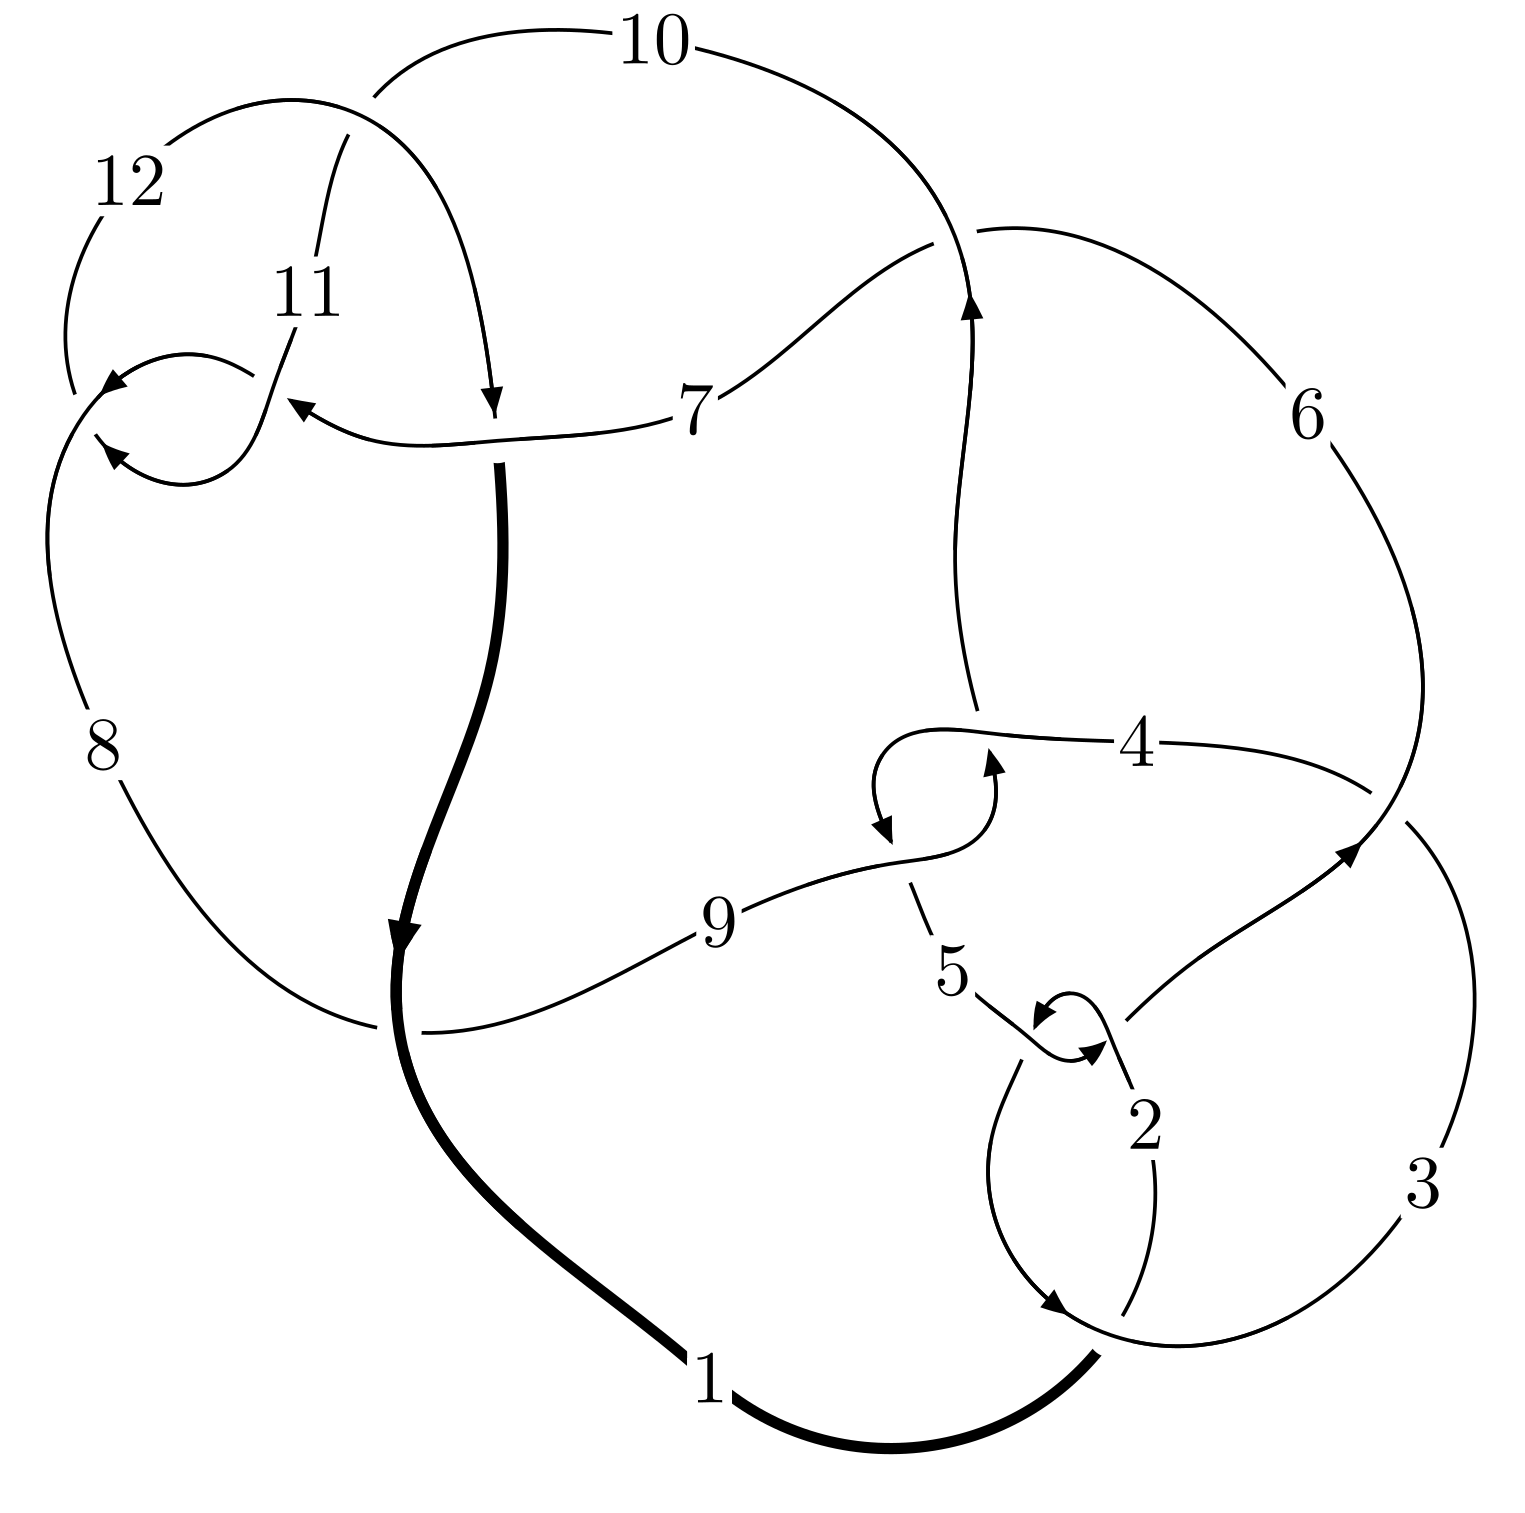
\includegraphics[width=112pt]{../../../GIT/diagram.site/Diagrams/png/821_12a_0020.png}\\
\ \ \ A knot diagram\footnotemark}&
\allowdisplaybreaks
\textbf{Linearized knot diagam} \\
\cline{2-2}
 &
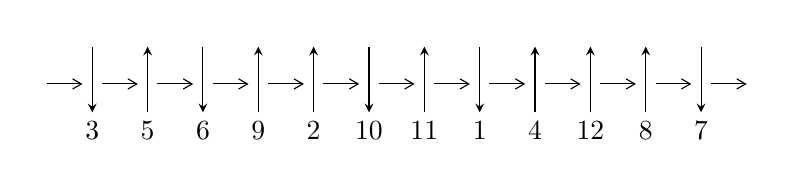
\begin{tikzpicture}[x=20pt, y=17pt]
	% nodes
	\node (C0) at (0, 0) {};
	\node (C1) at (1, 0) {};
	\node (C1U) at (1, +1) {};
	\node (C1D) at (1, -1) {3};

	\node (C2) at (2, 0) {};
	\node (C2U) at (2, +1) {};
	\node (C2D) at (2, -1) {5};

	\node (C3) at (3, 0) {};
	\node (C3U) at (3, +1) {};
	\node (C3D) at (3, -1) {6};

	\node (C4) at (4, 0) {};
	\node (C4U) at (4, +1) {};
	\node (C4D) at (4, -1) {9};

	\node (C5) at (5, 0) {};
	\node (C5U) at (5, +1) {};
	\node (C5D) at (5, -1) {2};

	\node (C6) at (6, 0) {};
	\node (C6U) at (6, +1) {};
	\node (C6D) at (6, -1) {10};

	\node (C7) at (7, 0) {};
	\node (C7U) at (7, +1) {};
	\node (C7D) at (7, -1) {11};

	\node (C8) at (8, 0) {};
	\node (C8U) at (8, +1) {};
	\node (C8D) at (8, -1) {1};

	\node (C9) at (9, 0) {};
	\node (C9U) at (9, +1) {};
	\node (C9D) at (9, -1) {4};

	\node (C10) at (10, 0) {};
	\node (C10U) at (10, +1) {};
	\node (C10D) at (10, -1) {12};

	\node (C11) at (11, 0) {};
	\node (C11U) at (11, +1) {};
	\node (C11D) at (11, -1) {8};

	\node (C12) at (12, 0) {};
	\node (C12U) at (12, +1) {};
	\node (C12D) at (12, -1) {7};
	\node (C13) at (13, 0) {};

	% arrows
	\draw[->,>={angle 60}]
	(C0) edge (C1) (C1) edge (C2) (C2) edge (C3) (C3) edge (C4) (C4) edge (C5) (C5) edge (C6) (C6) edge (C7) (C7) edge (C8) (C8) edge (C9) (C9) edge (C10) (C10) edge (C11) (C11) edge (C12) (C12) edge (C13) ;	\draw[->,>=stealth]
	(C1U) edge (C1D) (C2D) edge (C2U) (C3U) edge (C3D) (C4D) edge (C4U) (C5D) edge (C5U) (C6U) edge (C6D) (C7D) edge (C7U) (C8U) edge (C8D) (C9D) edge (C9U) (C10D) edge (C10U) (C11D) edge (C11U) (C12U) edge (C12D) ;
	\end{tikzpicture} \\
\hhline{~~} \\& 
\textbf{Solving Sequence} \\ \cline{2-2} 
 &
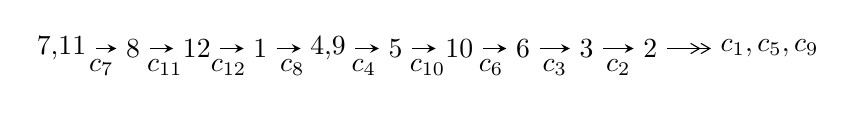
\begin{tikzpicture}[x=23pt, y=7pt]
	% node
	\node (A0) at (-1/8, 0) {7,11};
	\node (A1) at (1, 0) {8};
	\node (A2) at (2, 0) {12};
	\node (A3) at (3, 0) {1};
	\node (A4) at (65/16, 0) {4,9};
	\node (A5) at (41/8, 0) {5};
	\node (A6) at (49/8, 0) {10};
	\node (A7) at (57/8, 0) {6};
	\node (A8) at (65/8, 0) {3};
	\node (A9) at (73/8, 0) {2};
	\node (C1) at (1/2, -1) {$c_{7}$};
	\node (C2) at (3/2, -1) {$c_{11}$};
	\node (C3) at (5/2, -1) {$c_{12}$};
	\node (C4) at (7/2, -1) {$c_{8}$};
	\node (C5) at (37/8, -1) {$c_{4}$};
	\node (C6) at (45/8, -1) {$c_{10}$};
	\node (C7) at (53/8, -1) {$c_{6}$};
	\node (C8) at (61/8, -1) {$c_{3}$};
	\node (C9) at (69/8, -1) {$c_{2}$};
	\node (A10) at (11, 0) {$c_{1},c_{5},c_{9}$};

	% edge
	\draw[->,>=stealth]	
	(A0) edge (A1) (A1) edge (A2) (A2) edge (A3) (A3) edge (A4) (A4) edge (A5) (A5) edge (A6) (A6) edge (A7) (A7) edge (A8) (A8) edge (A9) ;
	\draw[->>,>={angle 60}]	
	(A9) edge (A10);
\end{tikzpicture} \\ 

\end{tabular} \\

\footnotetext{
The image of knot diagram is generated by the software ``\textbf{Draw programme}" developed by Andrew Bartholomew(\url{http://www.layer8.co.uk/maths/draw/index.htm\#Running-draw}), where we modified some parts for our purpose(\url{https://github.com/CATsTAILs/LinksPainter}).
}\phantom \\ \newline 
\centering \textbf{Ideals for irreducible components\footnotemark of $X_{\text{par}}$} 
 
\begin{align*}
I^u_{1}&=\langle 
10 u^{107}+12 u^{106}+\cdots+2 b+3 u,\;-2 u^{107}+4 u^{106}+\cdots+2 a+5,\;u^{108}+3 u^{107}+\cdots+2 u+1\rangle \\
I^u_{2}&=\langle 
- u^5 a+2 u^3 a-2 a u+b,\;u^4 a+u^5- u^4- u^2 a- u^3+a^2+a u+u^2- u,\;u^6- u^5- u^4+2 u^3- u+1\rangle \\
\\
\end{align*}
\raggedright * 2 irreducible components of $\dim_{\mathbb{C}}=0$, with total 120 representations.\\
\footnotetext{All coefficients of polynomials are rational numbers. But the coefficients are sometimes approximated in decimal forms when there is not enough margin.}
\newpage
\renewcommand{\arraystretch}{1}
\centering \section*{I. $I^u_{1}= \langle 10 u^{107}+12 u^{106}+\cdots+2 b+3 u,\;-2 u^{107}+4 u^{106}+\cdots+2 a+5,\;u^{108}+3 u^{107}+\cdots+2 u+1 \rangle$}
\flushleft \textbf{(i) Arc colorings}\\
\begin{tabular}{m{7pt} m{180pt} m{7pt} m{180pt} }
\flushright $a_{7}=$&$\begin{pmatrix}1\\0\end{pmatrix}$ \\
\flushright $a_{11}=$&$\begin{pmatrix}0\\u\end{pmatrix}$ \\
\flushright $a_{8}=$&$\begin{pmatrix}1\\- u^2\end{pmatrix}$ \\
\flushright $a_{12}=$&$\begin{pmatrix}u\\- u^3+u\end{pmatrix}$ \\
\flushright $a_{1}=$&$\begin{pmatrix}u^3\\- u^3+u\end{pmatrix}$ \\
\flushright $a_{4}=$&$\begin{pmatrix}u^{107}-2 u^{106}+\cdots-2 u-\frac{5}{2}\\-5 u^{107}-6 u^{106}+\cdots-2 u^2-\frac{3}{2} u\end{pmatrix}$ \\
\flushright $a_{9}=$&$\begin{pmatrix}u^8- u^6+u^4+1\\- u^8+2 u^6-2 u^4\end{pmatrix}$ \\
\flushright $a_{5}=$&$\begin{pmatrix}u^{107}+3 u^{106}+\cdots- u^2+\frac{1}{2}\\- u^{107}-3 u^{106}+\cdots-\frac{1}{2} u-1\end{pmatrix}$ \\
\flushright $a_{10}=$&$\begin{pmatrix}- u^3\\u^5- u^3+u\end{pmatrix}$ \\
\flushright $a_{6}=$&$\begin{pmatrix}u^8- u^6+u^4+1\\- u^{10}+2 u^8-3 u^6+2 u^4- u^2\end{pmatrix}$ \\
\flushright $a_{3}=$&$\begin{pmatrix}-\frac{1}{2} u^{107}-\frac{5}{2} u^{106}+\cdots-2 u-\frac{3}{2}\\-\frac{5}{2} u^{107}-\frac{7}{2} u^{106}+\cdots-\frac{1}{2} u^2-\frac{1}{2} u\end{pmatrix}$ \\
\flushright $a_{2}=$&$\begin{pmatrix}\frac{1}{2} u^{107}+\frac{3}{2} u^{106}+\cdots- u+\frac{3}{2}\\\frac{1}{2} u^{107}+\frac{1}{2} u^{106}+\cdots+\frac{3}{2} u^2+\frac{1}{2} u\end{pmatrix}$\\&\end{tabular}
\flushleft \textbf{(ii) Obstruction class $= -1$}\\~\\
\flushleft \textbf{(iii) Cusp Shapes $= 9 u^{107}+\frac{41}{2} u^{106}+\cdots+\frac{29}{2} u+14$}\\~\\
\newpage\renewcommand{\arraystretch}{1}
\flushleft \textbf{(iv) u-Polynomials at the component}\newline \\
\begin{tabular}{m{50pt}|m{274pt}}
Crossings & \hspace{64pt}u-Polynomials at each crossing \\
\hline $$\begin{aligned}c_{1}\end{aligned}$$&$\begin{aligned}
&u^{108}+55 u^{107}+\cdots+6 u+1
\end{aligned}$\\
\hline $$\begin{aligned}c_{2},c_{5}\end{aligned}$$&$\begin{aligned}
&u^{108}+7 u^{107}+\cdots+6 u+1
\end{aligned}$\\
\hline $$\begin{aligned}c_{3}\end{aligned}$$&$\begin{aligned}
&u^{108}-7 u^{107}+\cdots-83686 u+9881
\end{aligned}$\\
\hline $$\begin{aligned}c_{4},c_{9}\end{aligned}$$&$\begin{aligned}
&u^{108}+u^{107}+\cdots-4096 u+4096
\end{aligned}$\\
\hline $$\begin{aligned}c_{6},c_{8}\end{aligned}$$&$\begin{aligned}
&u^{108}+3 u^{107}+\cdots+5128 u+937
\end{aligned}$\\
\hline $$\begin{aligned}c_{7},c_{11}\end{aligned}$$&$\begin{aligned}
&u^{108}-3 u^{107}+\cdots-2 u+1
\end{aligned}$\\
\hline $$\begin{aligned}c_{10}\end{aligned}$$&$\begin{aligned}
&u^{108}-49 u^{107}+\cdots+2 u+1
\end{aligned}$\\
\hline $$\begin{aligned}c_{12}\end{aligned}$$&$\begin{aligned}
&u^{108}-9 u^{107}+\cdots-6 u+1
\end{aligned}$\\
\hline
\end{tabular}\\~\\
\newpage\renewcommand{\arraystretch}{1}
\flushleft \textbf{(v) Riley Polynomials at the component}\newline \\
\begin{tabular}{m{50pt}|m{274pt}}
Crossings & \hspace{64pt}Riley Polynomials at each crossing \\
\hline $$\begin{aligned}c_{1}\end{aligned}$$&$\begin{aligned}
&y^{108}+3 y^{107}+\cdots-10 y+1
\end{aligned}$\\
\hline $$\begin{aligned}c_{2},c_{5}\end{aligned}$$&$\begin{aligned}
&y^{108}+55 y^{107}+\cdots+6 y+1
\end{aligned}$\\
\hline $$\begin{aligned}c_{3}\end{aligned}$$&$\begin{aligned}
&y^{108}-49 y^{107}+\cdots+4881460918 y+97634161
\end{aligned}$\\
\hline $$\begin{aligned}c_{4},c_{9}\end{aligned}$$&$\begin{aligned}
&y^{108}+65 y^{107}+\cdots+385875968 y+16777216
\end{aligned}$\\
\hline $$\begin{aligned}c_{6},c_{8}\end{aligned}$$&$\begin{aligned}
&y^{108}-89 y^{107}+\cdots+14791066 y+877969
\end{aligned}$\\
\hline $$\begin{aligned}c_{7},c_{11}\end{aligned}$$&$\begin{aligned}
&y^{108}-49 y^{107}+\cdots+2 y+1
\end{aligned}$\\
\hline $$\begin{aligned}c_{10}\end{aligned}$$&$\begin{aligned}
&y^{108}+23 y^{107}+\cdots-26 y+1
\end{aligned}$\\
\hline $$\begin{aligned}c_{12}\end{aligned}$$&$\begin{aligned}
&y^{108}+3 y^{107}+\cdots+94 y+1
\end{aligned}$\\
\hline
\end{tabular}\\~\\
\newpage\flushleft \textbf{(vi) Complex Volumes and Cusp Shapes}
$$\begin{array}{c|c|c}  
\text{Solutions to }I^u_{1}& \I (\text{vol} + \sqrt{-1}CS) & \text{Cusp shape}\\
 \hline 
\begin{aligned}
u &= \phantom{-}0.988339 + 0.107184 I \\
a &= \phantom{-}0.20534 - 3.12417 I \\
b &= -0.24956 + 2.07122 I\end{aligned}
 & \phantom{-}1.31506 - 2.48598 I & \phantom{-0.000000 } 0 \\ \hline\begin{aligned}
u &= \phantom{-}0.988339 - 0.107184 I \\
a &= \phantom{-}0.20534 + 3.12417 I \\
b &= -0.24956 - 2.07122 I\end{aligned}
 & \phantom{-}1.31506 + 2.48598 I & \phantom{-0.000000 } 0 \\ \hline\begin{aligned}
u &= -0.967418 + 0.159869 I \\
a &= -0.859819 + 0.010363 I \\
b &= -0.031401 - 0.140629 I\end{aligned}
 & \phantom{-}1.66899 - 0.19592 I & \phantom{-0.000000 } 0 \\ \hline\begin{aligned}
u &= -0.967418 - 0.159869 I \\
a &= -0.859819 - 0.010363 I \\
b &= -0.031401 + 0.140629 I\end{aligned}
 & \phantom{-}1.66899 + 0.19592 I & \phantom{-0.000000 } 0 \\ \hline\begin{aligned}
u &= \phantom{-}0.834620 + 0.590673 I \\
a &= \phantom{-}0.995057 - 0.653328 I \\
b &= -0.837578 + 0.240181 I\end{aligned}
 & -5.60803 + 6.51271 I & \phantom{-0.000000 } 0 \\ \hline\begin{aligned}
u &= \phantom{-}0.834620 - 0.590673 I \\
a &= \phantom{-}0.995057 + 0.653328 I \\
b &= -0.837578 - 0.240181 I\end{aligned}
 & -5.60803 - 6.51271 I & \phantom{-0.000000 } 0 \\ \hline\begin{aligned}
u &= \phantom{-}0.797793 + 0.543102 I \\
a &= -1.000890 + 0.764090 I \\
b &= \phantom{-}0.838772 - 0.300099 I\end{aligned}
 & -2.40675 + 2.20833 I & \phantom{-0.000000 } 0 \\ \hline\begin{aligned}
u &= \phantom{-}0.797793 - 0.543102 I \\
a &= -1.000890 - 0.764090 I \\
b &= \phantom{-}0.838772 + 0.300099 I\end{aligned}
 & -2.40675 - 2.20833 I & \phantom{-0.000000 } 0 \\ \hline\begin{aligned}
u &= -0.937647 + 0.442291 I \\
a &= -0.915958 - 0.979918 I \\
b &= \phantom{-}0.485712 - 0.557097 I\end{aligned}
 & -0.059953 - 0.675856 I & \phantom{-0.000000 } 0 \\ \hline\begin{aligned}
u &= -0.937647 - 0.442291 I \\
a &= -0.915958 + 0.979918 I \\
b &= \phantom{-}0.485712 + 0.557097 I\end{aligned}
 & -0.059953 + 0.675856 I & \phantom{-0.000000 } 0\\
 \hline 
 \end{array}$$\newpage$$\begin{array}{c|c|c}  
\text{Solutions to }I^u_{1}& \I (\text{vol} + \sqrt{-1}CS) & \text{Cusp shape}\\
 \hline 
\begin{aligned}
u &= \phantom{-}0.752108 + 0.599057 I \\
a &= \phantom{-}0.881626 - 0.698045 I \\
b &= -0.769955 + 0.256180 I\end{aligned}
 & -5.84312 - 1.80068 I & \phantom{-0.000000 } 0 \\ \hline\begin{aligned}
u &= \phantom{-}0.752108 - 0.599057 I \\
a &= \phantom{-}0.881626 + 0.698045 I \\
b &= -0.769955 - 0.256180 I\end{aligned}
 & -5.84312 + 1.80068 I & \phantom{-0.000000 } 0 \\ \hline\begin{aligned}
u &= -1.048630 + 0.065579 I \\
a &= \phantom{-}1.014810 - 0.064670 I \\
b &= -0.0456004 + 0.0695150 I\end{aligned}
 & -0.80156 + 3.69498 I & \phantom{-0.000000 } 0 \\ \hline\begin{aligned}
u &= -1.048630 - 0.065579 I \\
a &= \phantom{-}1.014810 + 0.064670 I \\
b &= -0.0456004 - 0.0695150 I\end{aligned}
 & -0.80156 - 3.69498 I & \phantom{-0.000000 } 0 \\ \hline\begin{aligned}
u &= -0.551942 + 0.764427 I \\
a &= -0.366870 - 0.394614 I \\
b &= -0.51126 - 2.36364 I\end{aligned}
 & -10.22170 - 8.99067 I & \phantom{-0.000000 } 0 \\ \hline\begin{aligned}
u &= -0.551942 - 0.764427 I \\
a &= -0.366870 + 0.394614 I \\
b &= -0.51126 + 2.36364 I\end{aligned}
 & -10.22170 + 8.99067 I & \phantom{-0.000000 } 0 \\ \hline\begin{aligned}
u &= -0.524067 + 0.778480 I \\
a &= -0.197190 - 0.391437 I \\
b &= -0.42329 - 2.47740 I\end{aligned}
 & -12.01040 - 0.00877 I & \phantom{-0.000000 } 0 \\ \hline\begin{aligned}
u &= -0.524067 - 0.778480 I \\
a &= -0.197190 + 0.391437 I \\
b &= -0.42329 + 2.47740 I\end{aligned}
 & -12.01040 + 0.00877 I & \phantom{-0.000000 } 0 \\ \hline\begin{aligned}
u &= -0.536878 + 0.758750 I \\
a &= \phantom{-}0.311119 + 0.462328 I \\
b &= \phantom{-}0.53558 + 2.43939 I\end{aligned}
 & -7.31333 - 3.79136 I & \phantom{-0.000000 } 0 \\ \hline\begin{aligned}
u &= -0.536878 - 0.758750 I \\
a &= \phantom{-}0.311119 - 0.462328 I \\
b &= \phantom{-}0.53558 - 2.43939 I\end{aligned}
 & -7.31333 + 3.79136 I & \phantom{-0.000000 } 0\\
 \hline 
 \end{array}$$\newpage$$\begin{array}{c|c|c}  
\text{Solutions to }I^u_{1}& \I (\text{vol} + \sqrt{-1}CS) & \text{Cusp shape}\\
 \hline 
\begin{aligned}
u &= -1.044580 + 0.241783 I \\
a &= -0.655670 + 0.285020 I \\
b &= -0.035666 - 0.180815 I\end{aligned}
 & \phantom{-}2.10315 - 0.31022 I & \phantom{-0.000000 } 0 \\ \hline\begin{aligned}
u &= -1.044580 - 0.241783 I \\
a &= -0.655670 - 0.285020 I \\
b &= -0.035666 + 0.180815 I\end{aligned}
 & \phantom{-}2.10315 + 0.31022 I & \phantom{-0.000000 } 0 \\ \hline\begin{aligned}
u &= -0.452511 + 0.800257 I \\
a &= -0.239198 + 0.312900 I \\
b &= \phantom{-}0.07676 + 2.59514 I\end{aligned}
 & -11.60770 + 3.17330 I & \phantom{-0.000000 } 0 \\ \hline\begin{aligned}
u &= -0.452511 - 0.800257 I \\
a &= -0.239198 - 0.312900 I \\
b &= \phantom{-}0.07676 - 2.59514 I\end{aligned}
 & -11.60770 - 3.17330 I & \phantom{-0.000000 } 0 \\ \hline\begin{aligned}
u &= -0.426624 + 0.803472 I \\
a &= -0.381367 + 0.257467 I \\
b &= -0.06243 + 2.56356 I\end{aligned}
 & -9.5204 + 12.0780 I & \phantom{-0.000000 } 0 \\ \hline\begin{aligned}
u &= -0.426624 - 0.803472 I \\
a &= -0.381367 - 0.257467 I \\
b &= -0.06243 - 2.56356 I\end{aligned}
 & -9.5204 - 12.0780 I & \phantom{-0.000000 } 0 \\ \hline\begin{aligned}
u &= -0.433605 + 0.793273 I \\
a &= \phantom{-}0.361449 - 0.328654 I \\
b &= \phantom{-}0.03502 - 2.63170 I\end{aligned}
 & -6.73934 + 6.79720 I & \phantom{-0.000000 } 0 \\ \hline\begin{aligned}
u &= -0.433605 - 0.793273 I \\
a &= \phantom{-}0.361449 + 0.328654 I \\
b &= \phantom{-}0.03502 + 2.63170 I\end{aligned}
 & -6.73934 - 6.79720 I & \phantom{-0.000000 } 0 \\ \hline\begin{aligned}
u &= \phantom{-}0.497033 + 0.754891 I \\
a &= \phantom{-}0.614359 - 0.156153 I \\
b &= -0.480925 - 0.147891 I\end{aligned}
 & -6.16699 + 2.54092 I & \phantom{-0.000000 } 0 \\ \hline\begin{aligned}
u &= \phantom{-}0.497033 - 0.754891 I \\
a &= \phantom{-}0.614359 + 0.156153 I \\
b &= -0.480925 + 0.147891 I\end{aligned}
 & -6.16699 - 2.54092 I & \phantom{-0.000000 } 0\\
 \hline 
 \end{array}$$\newpage$$\begin{array}{c|c|c}  
\text{Solutions to }I^u_{1}& \I (\text{vol} + \sqrt{-1}CS) & \text{Cusp shape}\\
 \hline 
\begin{aligned}
u &= \phantom{-}0.457000 + 0.770798 I \\
a &= \phantom{-}0.615967 - 0.040560 I \\
b &= -0.435430 - 0.245808 I\end{aligned}
 & -5.94478 - 5.41063 I & \phantom{-0.000000 } 0 \\ \hline\begin{aligned}
u &= \phantom{-}0.457000 - 0.770798 I \\
a &= \phantom{-}0.615967 + 0.040560 I \\
b &= -0.435430 + 0.245808 I\end{aligned}
 & -5.94478 + 5.41063 I & \phantom{-0.000000 } 0 \\ \hline\begin{aligned}
u &= \phantom{-}1.026670 + 0.410086 I \\
a &= -2.00347 - 0.66989 I \\
b &= \phantom{-}1.33945 + 0.72536 I\end{aligned}
 & \phantom{-}2.30803 + 0.05509 I & \phantom{-0.000000 } 0 \\ \hline\begin{aligned}
u &= \phantom{-}1.026670 - 0.410086 I \\
a &= -2.00347 + 0.66989 I \\
b &= \phantom{-}1.33945 - 0.72536 I\end{aligned}
 & \phantom{-}2.30803 - 0.05509 I & \phantom{-0.000000 } 0 \\ \hline\begin{aligned}
u &= \phantom{-}0.869165 + 0.189560 I \\
a &= -0.85733 + 2.63181 I \\
b &= \phantom{-}0.73493 - 1.59061 I\end{aligned}
 & \phantom{-}1.06021 + 2.51609 I & \phantom{-0.000000 } 0 \\ \hline\begin{aligned}
u &= \phantom{-}0.869165 - 0.189560 I \\
a &= -0.85733 - 2.63181 I \\
b &= \phantom{-}0.73493 + 1.59061 I\end{aligned}
 & \phantom{-}1.06021 - 2.51609 I & \phantom{-0.000000 } 0 \\ \hline\begin{aligned}
u &= \phantom{-}1.108960 + 0.099543 I \\
a &= -0.09536 - 3.10102 I \\
b &= -0.02184 + 2.18073 I\end{aligned}
 & -1.51543 - 4.71449 I & \phantom{-0.000000 } 0 \\ \hline\begin{aligned}
u &= \phantom{-}1.108960 - 0.099543 I \\
a &= -0.09536 + 3.10102 I \\
b &= -0.02184 - 2.18073 I\end{aligned}
 & -1.51543 + 4.71449 I & \phantom{-0.000000 } 0 \\ \hline\begin{aligned}
u &= -0.478822 + 0.740548 I \\
a &= -0.022517 + 0.755190 I \\
b &= \phantom{-}0.48035 + 2.91161 I\end{aligned}
 & -3.69289 - 1.39830 I & \phantom{-0.000000 } 0 \\ \hline\begin{aligned}
u &= -0.478822 - 0.740548 I \\
a &= -0.022517 - 0.755190 I \\
b &= \phantom{-}0.48035 - 2.91161 I\end{aligned}
 & -3.69289 + 1.39830 I & \phantom{-0.000000 } 0\\
 \hline 
 \end{array}$$\newpage$$\begin{array}{c|c|c}  
\text{Solutions to }I^u_{1}& \I (\text{vol} + \sqrt{-1}CS) & \text{Cusp shape}\\
 \hline 
\begin{aligned}
u &= \phantom{-}1.116760 + 0.064140 I \\
a &= \phantom{-}0.05616 + 3.05434 I \\
b &= \phantom{-}0.01639 - 2.14974 I\end{aligned}
 & -6.19982 - 1.21253 I & \phantom{-0.000000 } 0 \\ \hline\begin{aligned}
u &= \phantom{-}1.116760 - 0.064140 I \\
a &= \phantom{-}0.05616 - 3.05434 I \\
b &= \phantom{-}0.01639 + 2.14974 I\end{aligned}
 & -6.19982 + 1.21253 I & \phantom{-0.000000 } 0 \\ \hline\begin{aligned}
u &= -0.457550 + 0.751409 I \\
a &= \phantom{-}0.236739 - 0.678641 I \\
b &= -0.21064 - 2.95573 I\end{aligned}
 & -3.57274 + 4.07736 I & \phantom{-0.000000 } 0 \\ \hline\begin{aligned}
u &= -0.457550 - 0.751409 I \\
a &= \phantom{-}0.236739 + 0.678641 I \\
b &= -0.21064 + 2.95573 I\end{aligned}
 & -3.57274 - 4.07736 I & \phantom{-0.000000 } 0 \\ \hline\begin{aligned}
u &= \phantom{-}0.462710 + 0.738208 I \\
a &= -0.530312 + 0.083449 I \\
b &= \phantom{-}0.384425 + 0.173480 I\end{aligned}
 & -3.01039 - 1.29247 I & \phantom{-0.000000 } 0 \\ \hline\begin{aligned}
u &= \phantom{-}0.462710 - 0.738208 I \\
a &= -0.530312 - 0.083449 I \\
b &= \phantom{-}0.384425 - 0.173480 I\end{aligned}
 & -3.01039 + 1.29247 I & \phantom{-0.000000 } 0 \\ \hline\begin{aligned}
u &= \phantom{-}1.128480 + 0.105840 I \\
a &= \phantom{-}0.12861 + 3.07346 I \\
b &= \phantom{-}0.00014 - 2.18012 I\end{aligned}
 & -4.24611 - 9.87631 I & \phantom{-0.000000 } 0 \\ \hline\begin{aligned}
u &= \phantom{-}1.128480 - 0.105840 I \\
a &= \phantom{-}0.12861 - 3.07346 I \\
b &= \phantom{-}0.00014 + 2.18012 I\end{aligned}
 & -4.24611 + 9.87631 I & \phantom{-0.000000 } 0 \\ \hline\begin{aligned}
u &= -1.054520 + 0.425286 I \\
a &= \phantom{-}0.02547 + 1.55678 I \\
b &= -0.743927 - 0.167461 I\end{aligned}
 & \phantom{-}3.44403 - 1.96877 I & \phantom{-0.000000 } 0 \\ \hline\begin{aligned}
u &= -1.054520 - 0.425286 I \\
a &= \phantom{-}0.02547 - 1.55678 I \\
b &= -0.743927 + 0.167461 I\end{aligned}
 & \phantom{-}3.44403 + 1.96877 I & \phantom{-0.000000 } 0\\
 \hline 
 \end{array}$$\newpage$$\begin{array}{c|c|c}  
\text{Solutions to }I^u_{1}& \I (\text{vol} + \sqrt{-1}CS) & \text{Cusp shape}\\
 \hline 
\begin{aligned}
u &= -1.082350 + 0.361078 I \\
a &= -0.406048 + 1.061330 I \\
b &= -0.356347 - 0.288763 I\end{aligned}
 & \phantom{-}3.04102 - 0.79102 I & \phantom{-0.000000 } 0 \\ \hline\begin{aligned}
u &= -1.082350 - 0.361078 I \\
a &= -0.406048 - 1.061330 I \\
b &= -0.356347 + 0.288763 I\end{aligned}
 & \phantom{-}3.04102 + 0.79102 I & \phantom{-0.000000 } 0 \\ \hline\begin{aligned}
u &= \phantom{-}1.055980 + 0.435500 I \\
a &= \phantom{-}1.48474 + 0.83408 I \\
b &= -0.966630 - 0.789840 I\end{aligned}
 & \phantom{-}3.37664 + 4.82818 I & \phantom{-0.000000 } 0 \\ \hline\begin{aligned}
u &= \phantom{-}1.055980 - 0.435500 I \\
a &= \phantom{-}1.48474 - 0.83408 I \\
b &= -0.966630 + 0.789840 I\end{aligned}
 & \phantom{-}3.37664 - 4.82818 I & \phantom{-0.000000 } 0 \\ \hline\begin{aligned}
u &= -1.107020 + 0.288464 I \\
a &= \phantom{-}0.730521 - 0.673979 I \\
b &= \phantom{-}0.100273 + 0.303998 I\end{aligned}
 & \phantom{-}0.18939 - 3.61311 I & \phantom{-0.000000 } 0 \\ \hline\begin{aligned}
u &= -1.107020 - 0.288464 I \\
a &= \phantom{-}0.730521 + 0.673979 I \\
b &= \phantom{-}0.100273 - 0.303998 I\end{aligned}
 & \phantom{-}0.18939 + 3.61311 I & \phantom{-0.000000 } 0 \\ \hline\begin{aligned}
u &= -1.049990 + 0.462991 I \\
a &= -0.28819 - 1.98702 I \\
b &= \phantom{-}1.089180 + 0.102951 I\end{aligned}
 & \phantom{-}1.90914 - 6.50178 I & \phantom{-0.000000 } 0 \\ \hline\begin{aligned}
u &= -1.049990 - 0.462991 I \\
a &= -0.28819 + 1.98702 I \\
b &= \phantom{-}1.089180 - 0.102951 I\end{aligned}
 & \phantom{-}1.90914 + 6.50178 I & \phantom{-0.000000 } 0 \\ \hline\begin{aligned}
u &= \phantom{-}1.023410 + 0.546186 I \\
a &= -0.804419 + 0.096562 I \\
b &= \phantom{-}0.606488 + 0.057072 I\end{aligned}
 & -1.18178 + 4.66447 I & \phantom{-0.000000 } 0 \\ \hline\begin{aligned}
u &= \phantom{-}1.023410 - 0.546186 I \\
a &= -0.804419 - 0.096562 I \\
b &= \phantom{-}0.606488 - 0.057072 I\end{aligned}
 & -1.18178 - 4.66447 I & \phantom{-0.000000 } 0\\
 \hline 
 \end{array}$$\newpage$$\begin{array}{c|c|c}  
\text{Solutions to }I^u_{1}& \I (\text{vol} + \sqrt{-1}CS) & \text{Cusp shape}\\
 \hline 
\begin{aligned}
u &= -1.117090 + 0.347714 I \\
a &= \phantom{-}0.675053 - 1.029150 I \\
b &= \phantom{-}0.257952 + 0.406551 I\end{aligned}
 & \phantom{-}0.80958 + 3.52182 I & \phantom{-0.000000 } 0 \\ \hline\begin{aligned}
u &= -1.117090 - 0.347714 I \\
a &= \phantom{-}0.675053 + 1.029150 I \\
b &= \phantom{-}0.257952 - 0.406551 I\end{aligned}
 & \phantom{-}0.80958 - 3.52182 I & \phantom{-0.000000 } 0 \\ \hline\begin{aligned}
u &= \phantom{-}0.511663 + 0.629009 I \\
a &= -0.362759 + 0.473363 I \\
b &= \phantom{-}0.391931 - 0.156748 I\end{aligned}
 & -2.68687 - 0.04189 I & -5.54547 + 0.84190 I \\ \hline\begin{aligned}
u &= \phantom{-}0.511663 - 0.629009 I \\
a &= -0.362759 - 0.473363 I \\
b &= \phantom{-}0.391931 + 0.156748 I\end{aligned}
 & -2.68687 + 0.04189 I & -5.54547 - 0.84190 I \\ \hline\begin{aligned}
u &= \phantom{-}0.389256 + 0.701926 I \\
a &= -0.397271 - 0.182434 I \\
b &= \phantom{-}0.154841 + 0.297132 I\end{aligned}
 & -2.11119 - 1.85406 I & -3.33744 - 1.25523 I \\ \hline\begin{aligned}
u &= \phantom{-}0.389256 - 0.701926 I \\
a &= -0.397271 + 0.182434 I \\
b &= \phantom{-}0.154841 - 0.297132 I\end{aligned}
 & -2.11119 + 1.85406 I & -3.33744 + 1.25523 I \\ \hline\begin{aligned}
u &= \phantom{-}1.099150 + 0.476941 I \\
a &= \phantom{-}0.830949 + 0.926063 I \\
b &= -0.494700 - 0.791915 I\end{aligned}
 & \phantom{-}2.25735 + 6.50648 I & \phantom{-0.000000 } 0 \\ \hline\begin{aligned}
u &= \phantom{-}1.099150 - 0.476941 I \\
a &= \phantom{-}0.830949 - 0.926063 I \\
b &= -0.494700 + 0.791915 I\end{aligned}
 & \phantom{-}2.25735 - 6.50648 I & \phantom{-0.000000 } 0 \\ \hline\begin{aligned}
u &= -1.032600 + 0.634454 I \\
a &= \phantom{-}2.81115 - 0.01355 I \\
b &= -0.72549 + 2.22542 I\end{aligned}
 & -8.78937 + 3.70138 I & \phantom{-0.000000 } 0 \\ \hline\begin{aligned}
u &= -1.032600 - 0.634454 I \\
a &= \phantom{-}2.81115 + 0.01355 I \\
b &= -0.72549 - 2.22542 I\end{aligned}
 & -8.78937 - 3.70138 I & \phantom{-0.000000 } 0\\
 \hline 
 \end{array}$$\newpage$$\begin{array}{c|c|c}  
\text{Solutions to }I^u_{1}& \I (\text{vol} + \sqrt{-1}CS) & \text{Cusp shape}\\
 \hline 
\begin{aligned}
u &= -1.040190 + 0.625894 I \\
a &= -3.00802 + 0.00968 I \\
b &= \phantom{-}0.77809 - 2.31439 I\end{aligned}
 & -5.81437 - 1.45353 I & \phantom{-0.000000 } 0 \\ \hline\begin{aligned}
u &= -1.040190 - 0.625894 I \\
a &= -3.00802 - 0.00968 I \\
b &= \phantom{-}0.77809 + 2.31439 I\end{aligned}
 & -5.81437 + 1.45353 I & \phantom{-0.000000 } 0 \\ \hline\begin{aligned}
u &= -0.698347 + 0.358237 I \\
a &= \phantom{-}1.127800 + 0.430881 I \\
b &= \phantom{-}0.369052 + 0.542782 I\end{aligned}
 & -0.81865 - 2.91747 I & -1.24476 + 5.59463 I \\ \hline\begin{aligned}
u &= -0.698347 - 0.358237 I \\
a &= \phantom{-}1.127800 - 0.430881 I \\
b &= \phantom{-}0.369052 - 0.542782 I\end{aligned}
 & -0.81865 + 2.91747 I & -1.24476 - 5.59463 I \\ \hline\begin{aligned}
u &= \phantom{-}1.120410 + 0.482009 I \\
a &= -0.669711 - 1.057560 I \\
b &= \phantom{-}0.364772 + 0.872661 I\end{aligned}
 & -0.08336 + 11.18210 I & \phantom{-0.000000 } 0 \\ \hline\begin{aligned}
u &= \phantom{-}1.120410 - 0.482009 I \\
a &= -0.669711 + 1.057560 I \\
b &= \phantom{-}0.364772 - 0.872661 I\end{aligned}
 & -0.08336 - 11.18210 I & \phantom{-0.000000 } 0 \\ \hline\begin{aligned}
u &= -1.068110 + 0.600311 I \\
a &= -4.01284 + 0.40577 I \\
b &= \phantom{-}0.78950 - 2.92246 I\end{aligned}
 & -1.94413 - 3.70964 I & \phantom{-0.000000 } 0 \\ \hline\begin{aligned}
u &= -1.068110 - 0.600311 I \\
a &= -4.01284 - 0.40577 I \\
b &= \phantom{-}0.78950 + 2.92246 I\end{aligned}
 & -1.94413 + 3.70964 I & \phantom{-0.000000 } 0 \\ \hline\begin{aligned}
u &= \phantom{-}1.061890 + 0.611912 I \\
a &= \phantom{-}0.531543 - 0.542681 I \\
b &= -0.491899 + 0.322984 I\end{aligned}
 & -4.48699 + 2.64493 I & \phantom{-0.000000 } 0 \\ \hline\begin{aligned}
u &= \phantom{-}1.061890 - 0.611912 I \\
a &= \phantom{-}0.531543 + 0.542681 I \\
b &= -0.491899 - 0.322984 I\end{aligned}
 & -4.48699 - 2.64493 I & \phantom{-0.000000 } 0\\
 \hline 
 \end{array}$$\newpage$$\begin{array}{c|c|c}  
\text{Solutions to }I^u_{1}& \I (\text{vol} + \sqrt{-1}CS) & \text{Cusp shape}\\
 \hline 
\begin{aligned}
u &= \phantom{-}1.107430 + 0.525741 I \\
a &= -0.378155 - 0.742703 I \\
b &= \phantom{-}0.180566 + 0.609014 I\end{aligned}
 & -1.37622 + 3.88574 I & \phantom{-0.000000 } 0 \\ \hline\begin{aligned}
u &= \phantom{-}1.107430 - 0.525741 I \\
a &= -0.378155 + 0.742703 I \\
b &= \phantom{-}0.180566 - 0.609014 I\end{aligned}
 & -1.37622 - 3.88574 I & \phantom{-0.000000 } 0 \\ \hline\begin{aligned}
u &= -1.053790 + 0.633254 I \\
a &= \phantom{-}3.02840 - 0.29418 I \\
b &= -0.65056 + 2.38910 I\end{aligned}
 & -10.43010 - 5.31401 I & \phantom{-0.000000 } 0 \\ \hline\begin{aligned}
u &= -1.053790 - 0.633254 I \\
a &= \phantom{-}3.02840 + 0.29418 I \\
b &= -0.65056 - 2.38910 I\end{aligned}
 & -10.43010 + 5.31401 I & \phantom{-0.000000 } 0 \\ \hline\begin{aligned}
u &= \phantom{-}1.075240 + 0.596163 I \\
a &= -0.397157 + 0.515456 I \\
b &= \phantom{-}0.382403 - 0.326592 I\end{aligned}
 & -1.19587 + 6.37964 I & \phantom{-0.000000 } 0 \\ \hline\begin{aligned}
u &= \phantom{-}1.075240 - 0.596163 I \\
a &= -0.397157 - 0.515456 I \\
b &= \phantom{-}0.382403 + 0.326592 I\end{aligned}
 & -1.19587 - 6.37964 I & \phantom{-0.000000 } 0 \\ \hline\begin{aligned}
u &= \phantom{-}1.091960 + 0.564968 I \\
a &= -0.032708 + 0.491605 I \\
b &= \phantom{-}0.098167 - 0.365521 I\end{aligned}
 & -0.06187 + 6.72615 I & \phantom{-0.000000 } 0 \\ \hline\begin{aligned}
u &= \phantom{-}1.091960 - 0.564968 I \\
a &= -0.032708 - 0.491605 I \\
b &= \phantom{-}0.098167 + 0.365521 I\end{aligned}
 & -0.06187 - 6.72615 I & \phantom{-0.000000 } 0 \\ \hline\begin{aligned}
u &= -1.080130 + 0.600513 I \\
a &= \phantom{-}3.97930 - 0.92607 I \\
b &= -0.48877 + 3.00058 I\end{aligned}
 & -1.72700 - 9.21242 I & \phantom{-0.000000 } 0 \\ \hline\begin{aligned}
u &= -1.080130 - 0.600513 I \\
a &= \phantom{-}3.97930 + 0.92607 I \\
b &= -0.48877 - 3.00058 I\end{aligned}
 & -1.72700 + 9.21242 I & \phantom{-0.000000 } 0\\
 \hline 
 \end{array}$$\newpage$$\begin{array}{c|c|c}  
\text{Solutions to }I^u_{1}& \I (\text{vol} + \sqrt{-1}CS) & \text{Cusp shape}\\
 \hline 
\begin{aligned}
u &= \phantom{-}1.085240 + 0.608507 I \\
a &= \phantom{-}0.413916 - 0.625299 I \\
b &= -0.414662 + 0.409632 I\end{aligned}
 & -4.07755 + 10.62320 I & \phantom{-0.000000 } 0 \\ \hline\begin{aligned}
u &= \phantom{-}1.085240 - 0.608507 I \\
a &= \phantom{-}0.413916 + 0.625299 I \\
b &= -0.414662 - 0.409632 I\end{aligned}
 & -4.07755 - 10.62320 I & \phantom{-0.000000 } 0 \\ \hline\begin{aligned}
u &= -1.095970 + 0.619592 I \\
a &= -3.26100 + 1.13443 I \\
b &= \phantom{-}0.26764 - 2.62651 I\end{aligned}
 & -9.68717 - 8.50119 I & \phantom{-0.000000 } 0 \\ \hline\begin{aligned}
u &= -1.095970 - 0.619592 I \\
a &= -3.26100 - 1.13443 I \\
b &= \phantom{-}0.26764 + 2.62651 I\end{aligned}
 & -9.68717 + 8.50119 I & \phantom{-0.000000 } 0 \\ \hline\begin{aligned}
u &= -1.101570 + 0.610511 I \\
a &= \phantom{-}3.34675 - 1.36341 I \\
b &= -0.14641 + 2.69917 I\end{aligned}
 & -4.75007 - 12.07200 I & \phantom{-0.000000 } 0 \\ \hline\begin{aligned}
u &= -1.101570 - 0.610511 I \\
a &= \phantom{-}3.34675 + 1.36341 I \\
b &= -0.14641 - 2.69917 I\end{aligned}
 & -4.75007 + 12.07200 I & \phantom{-0.000000 } 0 \\ \hline\begin{aligned}
u &= -1.107590 + 0.612193 I \\
a &= -3.21768 + 1.42770 I \\
b &= \phantom{-}0.09604 - 2.62944 I\end{aligned}
 & -7.4896 - 17.3843 I & \phantom{-0.000000 } 0 \\ \hline\begin{aligned}
u &= -1.107590 - 0.612193 I \\
a &= -3.21768 - 1.42770 I \\
b &= \phantom{-}0.09604 + 2.62944 I\end{aligned}
 & -7.4896 + 17.3843 I & \phantom{-0.000000 } 0 \\ \hline\begin{aligned}
u &= \phantom{-}0.257089 + 0.683772 I \\
a &= \phantom{-}0.583247 + 0.481691 I \\
b &= -0.030182 - 0.587958 I\end{aligned}
 & -3.78122 + 0.71131 I & -5.20307 - 0.83911 I \\ \hline\begin{aligned}
u &= \phantom{-}0.257089 - 0.683772 I \\
a &= \phantom{-}0.583247 - 0.481691 I \\
b &= -0.030182 + 0.587958 I\end{aligned}
 & -3.78122 - 0.71131 I & -5.20307 + 0.83911 I\\
 \hline 
 \end{array}$$\newpage$$\begin{array}{c|c|c}  
\text{Solutions to }I^u_{1}& \I (\text{vol} + \sqrt{-1}CS) & \text{Cusp shape}\\
 \hline 
\begin{aligned}
u &= \phantom{-}0.153738 + 0.674862 I \\
a &= \phantom{-}0.723502 + 0.567742 I \\
b &= \phantom{-}0.063780 - 0.743560 I\end{aligned}
 & -2.80986 - 6.85600 I & -2.41598 + 6.59324 I \\ \hline\begin{aligned}
u &= \phantom{-}0.153738 - 0.674862 I \\
a &= \phantom{-}0.723502 - 0.567742 I \\
b &= \phantom{-}0.063780 + 0.743560 I\end{aligned}
 & -2.80986 + 6.85600 I & -2.41598 - 6.59324 I \\ \hline\begin{aligned}
u &= \phantom{-}0.166199 + 0.612098 I \\
a &= -0.685708 - 0.657129 I \\
b &= -0.135776 + 0.672803 I\end{aligned}
 & -0.30433 - 2.34199 I & \phantom{-}1.24572 + 3.48957 I \\ \hline\begin{aligned}
u &= \phantom{-}0.166199 - 0.612098 I \\
a &= -0.685708 + 0.657129 I \\
b &= -0.135776 - 0.672803 I\end{aligned}
 & -0.30433 + 2.34199 I & \phantom{-}1.24572 - 3.48957 I \\ \hline\begin{aligned}
u &= -0.201548 + 0.404834 I \\
a &= \phantom{-}1.36434 + 0.67991 I \\
b &= \phantom{-}0.746393 - 0.428336 I\end{aligned}
 & -0.21644 + 2.77389 I & \phantom{-}2.22668 - 2.59702 I \\ \hline\begin{aligned}
u &= -0.201548 - 0.404834 I \\
a &= \phantom{-}1.36434 - 0.67991 I \\
b &= \phantom{-}0.746393 + 0.428336 I\end{aligned}
 & -0.21644 - 2.77389 I & \phantom{-}2.22668 + 2.59702 I \\ \hline\begin{aligned}
u &= \phantom{-}0.012805 + 0.441107 I \\
a &= -1.030300 - 0.907888 I \\
b &= -0.403676 + 0.591229 I\end{aligned}
 & \phantom{-}0.90929 - 1.38472 I & \phantom{-}4.15458 + 4.07736 I \\ \hline\begin{aligned}
u &= \phantom{-}0.012805 - 0.441107 I \\
a &= -1.030300 + 0.907888 I \\
b &= -0.403676 - 0.591229 I\end{aligned}
 & \phantom{-}0.90929 + 1.38472 I & \phantom{-}4.15458 - 4.07736 I\\
 \hline 
 \end{array}$$\newpage\newpage\renewcommand{\arraystretch}{1}
\centering \section*{II. $I^u_{2}= \langle - u^5 a+2 u^3 a-2 a u+b,\;u^4 a+u^5- u^4- u^2 a- u^3+a^2+a u+u^2- u,\;u^6- u^5- u^4+2 u^3- u+1 \rangle$}
\flushleft \textbf{(i) Arc colorings}\\
\begin{tabular}{m{7pt} m{180pt} m{7pt} m{180pt} }
\flushright $a_{7}=$&$\begin{pmatrix}1\\0\end{pmatrix}$ \\
\flushright $a_{11}=$&$\begin{pmatrix}0\\u\end{pmatrix}$ \\
\flushright $a_{8}=$&$\begin{pmatrix}1\\- u^2\end{pmatrix}$ \\
\flushright $a_{12}=$&$\begin{pmatrix}u\\- u^3+u\end{pmatrix}$ \\
\flushright $a_{1}=$&$\begin{pmatrix}u^3\\- u^3+u\end{pmatrix}$ \\
\flushright $a_{4}=$&$\begin{pmatrix}a\\u^5 a-2 u^3 a+2 a u\end{pmatrix}$ \\
\flushright $a_{9}=$&$\begin{pmatrix}- u^3\\u^5- u^3+u\end{pmatrix}$ \\
\flushright $a_{5}=$&$\begin{pmatrix}a\\u^5 a-2 u^3 a+2 a u\end{pmatrix}$ \\
\flushright $a_{10}=$&$\begin{pmatrix}- u^3\\u^5- u^3+u\end{pmatrix}$ \\
\flushright $a_{6}=$&$\begin{pmatrix}- u^3\\u^3- u\end{pmatrix}$ \\
\flushright $a_{3}=$&$\begin{pmatrix}u^5 a- u^3 a+a u+a\\- u^5 a+u^4 a+u^3 a-2 u^2 a+a\end{pmatrix}$ \\
\flushright $a_{2}=$&$\begin{pmatrix}u^5 a- u^3 a+u^4+a u- u^2+a+u\\- u^5 a+u^4 a+u^3 a-2 u^2 a+a+1\end{pmatrix}$\\&\end{tabular}
\flushleft \textbf{(ii) Obstruction class $= 1$}\\~\\
\flushleft \textbf{(iii) Cusp Shapes $= -6 u^5 a+2 u^4 a+10 u^3 a-4 u^4-3 u^2 a+u^3-9 a u+3 u^2+2 a-4 u-1$}\\~\\
\newpage\renewcommand{\arraystretch}{1}
\flushleft \textbf{(iv) u-Polynomials at the component}\newline \\
\begin{tabular}{m{50pt}|m{274pt}}
Crossings & \hspace{64pt}u-Polynomials at each crossing \\
\hline $$\begin{aligned}c_{1},c_{3},c_{5}\end{aligned}$$&$\begin{aligned}
&(u^2- u+1)^6
\end{aligned}$\\
\hline $$\begin{aligned}c_{2}\end{aligned}$$&$\begin{aligned}
&(u^2+u+1)^6
\end{aligned}$\\
\hline $$\begin{aligned}c_{4},c_{9}\end{aligned}$$&$\begin{aligned}
&u^{12}
\end{aligned}$\\
\hline $$\begin{aligned}c_{6},c_{8},c_{11}\end{aligned}$$&$\begin{aligned}
&(u^6+u^5- u^4-2 u^3+u+1)^2
\end{aligned}$\\
\hline $$\begin{aligned}c_{7}\end{aligned}$$&$\begin{aligned}
&(u^6- u^5- u^4+2 u^3- u+1)^2
\end{aligned}$\\
\hline $$\begin{aligned}c_{10},c_{12}\end{aligned}$$&$\begin{aligned}
&(u^6+3 u^5+5 u^4+4 u^3+2 u^2+u+1)^2
\end{aligned}$\\
\hline
\end{tabular}\\~\\
\newpage\renewcommand{\arraystretch}{1}
\flushleft \textbf{(v) Riley Polynomials at the component}\newline \\
\begin{tabular}{m{50pt}|m{274pt}}
Crossings & \hspace{64pt}Riley Polynomials at each crossing \\
\hline $$\begin{aligned}c_{1},c_{2},c_{3}\\c_{5}\end{aligned}$$&$\begin{aligned}
&(y^2+y+1)^6
\end{aligned}$\\
\hline $$\begin{aligned}c_{4},c_{9}\end{aligned}$$&$\begin{aligned}
&y^{12}
\end{aligned}$\\
\hline $$\begin{aligned}c_{6},c_{7},c_{8}\\c_{11}\end{aligned}$$&$\begin{aligned}
&(y^6-3 y^5+5 y^4-4 y^3+2 y^2- y+1)^2
\end{aligned}$\\
\hline $$\begin{aligned}c_{10},c_{12}\end{aligned}$$&$\begin{aligned}
&(y^6+y^5+5 y^4+6 y^2+3 y+1)^2
\end{aligned}$\\
\hline
\end{tabular}\\~\\
\newpage\flushleft \textbf{(vi) Complex Volumes and Cusp Shapes}
$$\begin{array}{c|c|c}  
\text{Solutions to }I^u_{2}& \I (\text{vol} + \sqrt{-1}CS) & \text{Cusp shape}\\
 \hline 
\begin{aligned}
u &= -1.002190 + 0.295542 I \\
a &= \phantom{-}0.54263 + 1.33698 I \\
b &= -0.500000 - 0.866025 I\end{aligned}
 & \phantom{-}1.89061 + 1.10558 I & \phantom{-}3.50232 - 2.57477 I \\ \hline\begin{aligned}
u &= -1.002190 + 0.295542 I \\
a &= \phantom{-}0.88654 - 1.13843 I \\
b &= -0.500000 + 0.866025 I\end{aligned}
 & \phantom{-}1.89061 - 2.95419 I & \phantom{-}7.01188 + 5.05114 I \\ \hline\begin{aligned}
u &= -1.002190 - 0.295542 I \\
a &= \phantom{-}0.54263 - 1.33698 I \\
b &= -0.500000 + 0.866025 I\end{aligned}
 & \phantom{-}1.89061 - 1.10558 I & \phantom{-}3.50232 + 2.57477 I \\ \hline\begin{aligned}
u &= -1.002190 - 0.295542 I \\
a &= \phantom{-}0.88654 + 1.13843 I \\
b &= -0.500000 - 0.866025 I\end{aligned}
 & \phantom{-}1.89061 + 2.95419 I & \phantom{-}7.01188 - 5.05114 I \\ \hline\begin{aligned}
u &= \phantom{-}0.428243 + 0.664531 I \\
a &= -0.386545 - 0.272402 I \\
b &= -0.500000 - 0.866025 I\end{aligned}
 & -1.89061 - 2.95419 I & -1.81693 + 4.43387 I \\ \hline\begin{aligned}
u &= \phantom{-}0.428243 + 0.664531 I \\
a &= -0.042635 + 0.470959 I \\
b &= -0.500000 + 0.866025 I\end{aligned}
 & -1.89061 + 1.10558 I & \phantom{-}0.06995 - 2.75005 I \\ \hline\begin{aligned}
u &= \phantom{-}0.428243 - 0.664531 I \\
a &= -0.386545 + 0.272402 I \\
b &= -0.500000 + 0.866025 I\end{aligned}
 & -1.89061 + 2.95419 I & -1.81693 - 4.43387 I \\ \hline\begin{aligned}
u &= \phantom{-}0.428243 - 0.664531 I \\
a &= -0.042635 - 0.470959 I \\
b &= -0.500000 - 0.866025 I\end{aligned}
 & -1.89061 - 1.10558 I & \phantom{-}0.06995 + 2.75005 I \\ \hline\begin{aligned}
u &= \phantom{-}1.073950 + 0.558752 I \\
a &= \phantom{-}1.44307 - 0.25581 I \\
b &= -0.500000 - 0.866025 I\end{aligned}
 & \phantom{-0.000000 -}7.72290 I & \phantom{-}1.09315 - 9.68468 I \\ \hline\begin{aligned}
u &= \phantom{-}1.073950 + 0.558752 I \\
a &= -0.94307 - 1.12183 I \\
b &= -0.500000 + 0.866025 I\end{aligned}
 & \phantom{-0.000000 -}3.66314 I & \phantom{-}4.13964 - 1.97785 I\\
 \hline 
 \end{array}$$\newpage$$\begin{array}{c|c|c}  
\text{Solutions to }I^u_{2}& \I (\text{vol} + \sqrt{-1}CS) & \text{Cusp shape}\\
 \hline 
\begin{aligned}
u &= \phantom{-}1.073950 - 0.558752 I \\
a &= \phantom{-}1.44307 + 0.25581 I \\
b &= -0.500000 + 0.866025 I\end{aligned}
 & \phantom{-0.000000 } -7.72290 I & \phantom{-}1.09315 + 9.68468 I \\ \hline\begin{aligned}
u &= \phantom{-}1.073950 - 0.558752 I \\
a &= -0.94307 + 1.12183 I \\
b &= -0.500000 - 0.866025 I\end{aligned}
 & \phantom{-0.000000 } -3.66314 I & \phantom{-}4.13964 + 1.97785 I\\
 \hline 
 \end{array}$$\newpage
\newpage\renewcommand{\arraystretch}{1}
\centering \section*{ III. u-Polynomials}
\begin{tabular}{m{50pt}|m{274pt}}
Crossings & \hspace{64pt}u-Polynomials at each crossing \\
\hline $$\begin{aligned}c_{1}\end{aligned}$$&$\begin{aligned}
&((u^2- u+1)^6)(u^{108}+55 u^{107}+\cdots+6 u+1)
\end{aligned}$\\
\hline $$\begin{aligned}c_{2}\end{aligned}$$&$\begin{aligned}
&((u^2+u+1)^6)(u^{108}+7 u^{107}+\cdots+6 u+1)
\end{aligned}$\\
\hline $$\begin{aligned}c_{3}\end{aligned}$$&$\begin{aligned}
&((u^2- u+1)^6)(u^{108}-7 u^{107}+\cdots-83686 u+9881)
\end{aligned}$\\
\hline $$\begin{aligned}c_{4},c_{9}\end{aligned}$$&$\begin{aligned}
&u^{12}(u^{108}+u^{107}+\cdots-4096 u+4096)
\end{aligned}$\\
\hline $$\begin{aligned}c_{5}\end{aligned}$$&$\begin{aligned}
&((u^2- u+1)^6)(u^{108}+7 u^{107}+\cdots+6 u+1)
\end{aligned}$\\
\hline $$\begin{aligned}c_{6},c_{8}\end{aligned}$$&$\begin{aligned}
&((u^6+u^5- u^4-2 u^3+u+1)^2)(u^{108}+3 u^{107}+\cdots+5128 u+937)
\end{aligned}$\\
\hline $$\begin{aligned}c_{7}\end{aligned}$$&$\begin{aligned}
&((u^6- u^5- u^4+2 u^3- u+1)^2)(u^{108}-3 u^{107}+\cdots-2 u+1)
\end{aligned}$\\
\hline $$\begin{aligned}c_{10}\end{aligned}$$&$\begin{aligned}
&((u^6+3 u^5+5 u^4+4 u^3+2 u^2+u+1)^{2})(u^{108}-49 u^{107}+\cdots+2 u+1)
\end{aligned}$\\
\hline $$\begin{aligned}c_{11}\end{aligned}$$&$\begin{aligned}
&((u^6+u^5- u^4-2 u^3+u+1)^2)(u^{108}-3 u^{107}+\cdots-2 u+1)
\end{aligned}$\\
\hline $$\begin{aligned}c_{12}\end{aligned}$$&$\begin{aligned}
&((u^6+3 u^5+5 u^4+4 u^3+2 u^2+u+1)^{2})(u^{108}-9 u^{107}+\cdots-6 u+1)
\end{aligned}$\\
\hline
\end{tabular}\newpage\renewcommand{\arraystretch}{1}
\centering \section*{ IV. Riley Polynomials}
\begin{tabular}{m{50pt}|m{274pt}}
Crossings & \hspace{64pt}Riley Polynomials at each crossing \\
\hline $$\begin{aligned}c_{1}\end{aligned}$$&$\begin{aligned}
&((y^2+y+1)^6)(y^{108}+3 y^{107}+\cdots-10 y+1)
\end{aligned}$\\
\hline $$\begin{aligned}c_{2},c_{5}\end{aligned}$$&$\begin{aligned}
&((y^2+y+1)^6)(y^{108}+55 y^{107}+\cdots+6 y+1)
\end{aligned}$\\
\hline $$\begin{aligned}c_{3}\end{aligned}$$&$\begin{aligned}
&((y^2+y+1)^6)(y^{108}-49 y^{107}+\cdots+4.88146\times10^{9} y+9.76342\times10^{7})
\end{aligned}$\\
\hline $$\begin{aligned}c_{4},c_{9}\end{aligned}$$&$\begin{aligned}
&y^{12}(y^{108}+65 y^{107}+\cdots+3.85876\times10^{8} y+1.67772\times10^{7})
\end{aligned}$\\
\hline $$\begin{aligned}c_{6},c_{8}\end{aligned}$$&$\begin{aligned}
&(y^6-3 y^5+5 y^4-4 y^3+2 y^2- y+1)^2\\
&\cdot(y^{108}-89 y^{107}+\cdots+14791066 y+877969)
\end{aligned}$\\
\hline $$\begin{aligned}c_{7},c_{11}\end{aligned}$$&$\begin{aligned}
&((y^6-3 y^5+5 y^4-4 y^3+2 y^2- y+1)^{2})(y^{108}-49 y^{107}+\cdots+2 y+1)
\end{aligned}$\\
\hline $$\begin{aligned}c_{10}\end{aligned}$$&$\begin{aligned}
&((y^6+y^5+5 y^4+6 y^2+3 y+1)^2)(y^{108}+23 y^{107}+\cdots-26 y+1)
\end{aligned}$\\
\hline $$\begin{aligned}c_{12}\end{aligned}$$&$\begin{aligned}
&((y^6+y^5+5 y^4+6 y^2+3 y+1)^2)(y^{108}+3 y^{107}+\cdots+94 y+1)
\end{aligned}$\\
\hline
\end{tabular}
\vskip 2pc
\end{document}